\section{Endereçamento aberto}

\begin{frame}{Problemas com a colisão} 

	\begin{itemize}
		\item Como visto, as funções de \textit{hash} podem gerar colisões, isto é, 
            um mesmo índice para duas chaves distintas

		\item Naturalmente surge o seguinte questionamento: como inserir duas chaves que colidem 
            em uma mesma tabela, e como resgatá-las em uma busca?

		\item Uma alternativa para o tratamento de colisões é o endereçamento aberto
	\end{itemize}

\end{frame}

\begin{frame}{Endereçamento aberto} 

    \metroset{block=fill}
    \begin{block}{Definição}
        Se a chave $K$ for mapeada para uma posição já ocupada da tabela, o 
        endereçamento aberto utiliza a sequência de sondagem
        $$
        N(h(K) + p(1)), N(h(K) + p(2)),  \ldots, N(h(K) + p(i)), \ldots
        $$
        onde $p$ é a função de sondagem, $i$ é o índice de sondagem e $N$ a função de 
        normalização, até que 
        \begin{enumerate}
            \item se encontre uma posição desocupada
            \item $N(h(K) + p(j)) = N(h(K))$
            \item se verifique que a tabela está cheia
        \end{enumerate}
    \end{block}

\end{frame}

\begin{frame}{Sondagem linear} 

	\begin{itemize}
		\item Na sondagem linear, temos a função de sondagem é a identidade, isto é,
            $p(i) = i, \forall i$

        \item A função de normalização faz com que o índice resultante esteja dentro dos 
            limites da tabela, usando o resto da divisão:
            \[
                N(K) = K (\mbox{mod}\ T), \]
            onde $T$ é o tamanho da tabela

		\item Se uma posição $N(h(K) + p(i))$ já estiver ocupada, tenta-se o próximo índice de 
            sondagem ($i + 1$) até que se encontre um espaço vago ou ocorra uma das outras 
            condições

		\item Esta estratégia tende a formação de agrupamentos de chaves, com pontos de 
            acumulação na tabela e intervalos contíguos não ocupados
	\end{itemize}

\end{frame}

\begin{frame}{Exemplo de inserção utilizando sondagem linear} 

    \begin{figure}
        \begin{tikzpicture}
            \draw (0, 1) grid (11, 2);

            \node at (0.5, 2.5) { \tt \footnotesize 0 };
            \node at (1.5, 2.5) { \tt \footnotesize 1 };
            \node at (2.5, 2.5) { \tt \footnotesize 2 };
            \node at (3.5, 2.5) { \tt \footnotesize 3 };
            \node at (4.5, 2.5) { \tt \footnotesize 4 };
            \node at (5.5, 2.5) { \tt \footnotesize 5 };
            \node at (6.5, 2.5) { \tt \footnotesize 6 };
            \node at (7.5, 2.5) { \tt \footnotesize 7 };
            \node at (8.5, 2.5) { \tt \footnotesize 8 };
            \node at (9.5, 2.5) { \tt \footnotesize 9 };
            \node at (10.5, 2.5) { \tt \footnotesize 10 };

            \node[anchor=west] at (1, 6) { Sondagem linear, $T = 11$ };
            \node[anchor=west] at (1, 5.5) { Elemento a ser inserido: \textcolor{blue}{$51$} };

        \end{tikzpicture}
    \end{figure}

\end{frame}

\begin{frame}{Exemplo de inserção utilizando sondagem linear} 

    \begin{figure}
        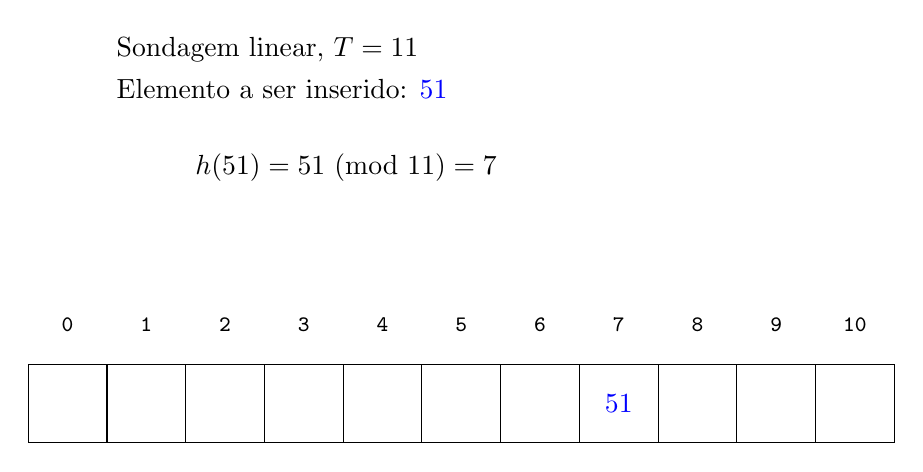
\begin{tikzpicture}
            \draw (0, 1) grid (11, 2);

            \node at (0.5, 2.5) { \tt \footnotesize 0 };
            \node at (1.5, 2.5) { \tt \footnotesize 1 };
            \node at (2.5, 2.5) { \tt \footnotesize 2 };
            \node at (3.5, 2.5) { \tt \footnotesize 3 };
            \node at (4.5, 2.5) { \tt \footnotesize 4 };
            \node at (5.5, 2.5) { \tt \footnotesize 5 };
            \node at (6.5, 2.5) { \tt \footnotesize 6 };
            \node at (7.5, 2.5) { \tt \footnotesize 7 };
            \node at (8.5, 2.5) { \tt \footnotesize 8 };
            \node at (9.5, 2.5) { \tt \footnotesize 9 };
            \node at (10.5, 2.5) { \tt \footnotesize 10 };

            \node[anchor=west] at (1, 6) { Sondagem linear, $T = 11$ };
            \node[anchor=west] at (1, 5.5) { Elemento a ser inserido: \textcolor{blue}{$51$} };

            \node[anchor=west] at (2, 4.5) { $h(51) = 51\ (\mbox{mod}\ 11) = 7$ };

            \node at (7.5, 1.5) { \textcolor{blue}{$51$} };
        \end{tikzpicture}
    \end{figure}

\end{frame}

\begin{frame}{Exemplo de inserção utilizando sondagem linear} 

    \begin{figure}
        \begin{tikzpicture}
            \draw (0, 1) grid (11, 2);

            \node at (0.5, 2.5) { \tt \footnotesize 0 };
            \node at (1.5, 2.5) { \tt \footnotesize 1 };
            \node at (2.5, 2.5) { \tt \footnotesize 2 };
            \node at (3.5, 2.5) { \tt \footnotesize 3 };
            \node at (4.5, 2.5) { \tt \footnotesize 4 };
            \node at (5.5, 2.5) { \tt \footnotesize 5 };
            \node at (6.5, 2.5) { \tt \footnotesize 6 };
            \node at (7.5, 2.5) { \tt \footnotesize 7 };
            \node at (8.5, 2.5) { \tt \footnotesize 8 };
            \node at (9.5, 2.5) { \tt \footnotesize 9 };
            \node at (10.5, 2.5) { \tt \footnotesize 10 };

            \node[anchor=west] at (1, 6) { Sondagem linear, $T = 11$ };
            \node[anchor=west] at (1, 5.5) { Elemento a ser inserido: \textcolor{blue}{$16$} };

%            \node[anchor=west] at (2, 4.5) { $h(51) = 51\ (\mbox{mod}\ 11) = 7$ };

            \node at (7.5, 1.5) { \textcolor{black}{$51$} };
        \end{tikzpicture}
    \end{figure}

\end{frame}

\begin{frame}{Exemplo de inserção utilizando sondagem linear} 

    \begin{figure}
        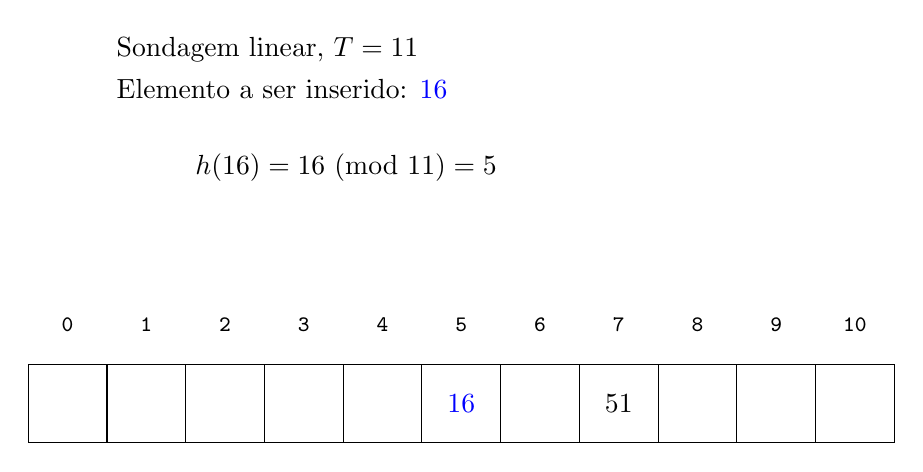
\begin{tikzpicture}
            \draw (0, 1) grid (11, 2);

            \node at (0.5, 2.5) { \tt \footnotesize 0 };
            \node at (1.5, 2.5) { \tt \footnotesize 1 };
            \node at (2.5, 2.5) { \tt \footnotesize 2 };
            \node at (3.5, 2.5) { \tt \footnotesize 3 };
            \node at (4.5, 2.5) { \tt \footnotesize 4 };
            \node at (5.5, 2.5) { \tt \footnotesize 5 };
            \node at (6.5, 2.5) { \tt \footnotesize 6 };
            \node at (7.5, 2.5) { \tt \footnotesize 7 };
            \node at (8.5, 2.5) { \tt \footnotesize 8 };
            \node at (9.5, 2.5) { \tt \footnotesize 9 };
            \node at (10.5, 2.5) { \tt \footnotesize 10 };

            \node[anchor=west] at (1, 6) { Sondagem linear, $T = 11$ };
            \node[anchor=west] at (1, 5.5) { Elemento a ser inserido: \textcolor{blue}{$16$} };

            \node[anchor=west] at (2, 4.5) { $h(16) = 16\ (\mbox{mod}\ 11) = 5$ };

            \node at (5.5, 1.5) { \textcolor{blue}{$16$} };
            \node at (7.5, 1.5) { \textcolor{black}{$51$} };
        \end{tikzpicture}
    \end{figure}

\end{frame}

\begin{frame}{Exemplo de inserção utilizando sondagem linear} 

    \begin{figure}
        \begin{tikzpicture}
            \draw (0, 1) grid (11, 2);

            \node at (0.5, 2.5) { \tt \footnotesize 0 };
            \node at (1.5, 2.5) { \tt \footnotesize 1 };
            \node at (2.5, 2.5) { \tt \footnotesize 2 };
            \node at (3.5, 2.5) { \tt \footnotesize 3 };
            \node at (4.5, 2.5) { \tt \footnotesize 4 };
            \node at (5.5, 2.5) { \tt \footnotesize 5 };
            \node at (6.5, 2.5) { \tt \footnotesize 6 };
            \node at (7.5, 2.5) { \tt \footnotesize 7 };
            \node at (8.5, 2.5) { \tt \footnotesize 8 };
            \node at (9.5, 2.5) { \tt \footnotesize 9 };
            \node at (10.5, 2.5) { \tt \footnotesize 10 };

            \node[anchor=west] at (1, 6) { Sondagem linear, $T = 11$ };
            \node[anchor=west] at (1, 5.5) { Elemento a ser inserido: \textcolor{blue}{$76$} };

%            \node[anchor=west] at (2, 4.5) { $h(16) = 16\ (\mbox{mod}\ 11) = 5$ };

            \node at (5.5, 1.5) { \textcolor{black}{$16$} };
            \node at (7.5, 1.5) { \textcolor{black}{$51$} };
        \end{tikzpicture}
    \end{figure}

\end{frame}

\begin{frame}{Exemplo de inserção utilizando sondagem linear} 

    \begin{figure}
        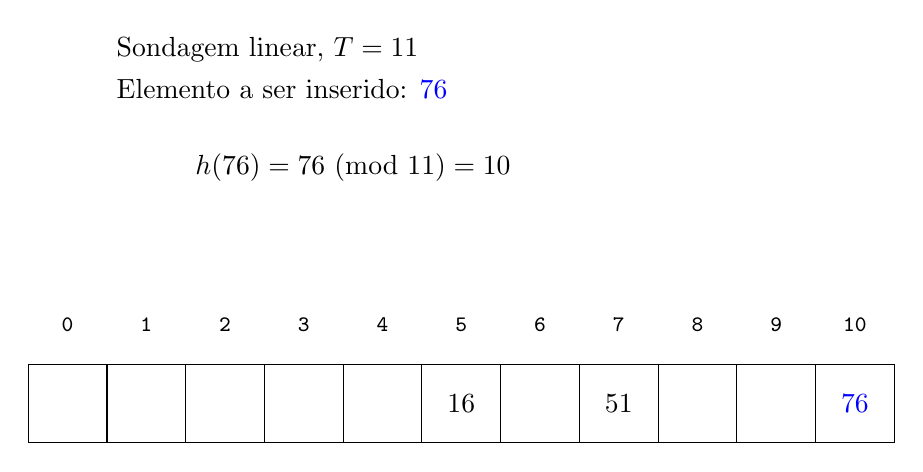
\begin{tikzpicture}
            \draw (0, 1) grid (11, 2);

            \node at (0.5, 2.5) { \tt \footnotesize 0 };
            \node at (1.5, 2.5) { \tt \footnotesize 1 };
            \node at (2.5, 2.5) { \tt \footnotesize 2 };
            \node at (3.5, 2.5) { \tt \footnotesize 3 };
            \node at (4.5, 2.5) { \tt \footnotesize 4 };
            \node at (5.5, 2.5) { \tt \footnotesize 5 };
            \node at (6.5, 2.5) { \tt \footnotesize 6 };
            \node at (7.5, 2.5) { \tt \footnotesize 7 };
            \node at (8.5, 2.5) { \tt \footnotesize 8 };
            \node at (9.5, 2.5) { \tt \footnotesize 9 };
            \node at (10.5, 2.5) { \tt \footnotesize 10 };

            \node[anchor=west] at (1, 6) { Sondagem linear, $T = 11$ };
            \node[anchor=west] at (1, 5.5) { Elemento a ser inserido: \textcolor{blue}{$76$} };

            \node[anchor=west] at (2, 4.5) { $h(76) = 76\ (\mbox{mod}\ 11) = 10$ };

            \node at (5.5, 1.5) { \textcolor{black}{$16$} };
            \node at (7.5, 1.5) { \textcolor{black}{$51$} };
            \node at (10.5, 1.5) { \textcolor{blue}{$76$} };
        \end{tikzpicture}
    \end{figure}

\end{frame}

\begin{frame}{Exemplo de inserção utilizando sondagem linear} 

    \begin{figure}
        \begin{tikzpicture}
            \draw (0, 1) grid (11, 2);

            \node at (0.5, 2.5) { \tt \footnotesize 0 };
            \node at (1.5, 2.5) { \tt \footnotesize 1 };
            \node at (2.5, 2.5) { \tt \footnotesize 2 };
            \node at (3.5, 2.5) { \tt \footnotesize 3 };
            \node at (4.5, 2.5) { \tt \footnotesize 4 };
            \node at (5.5, 2.5) { \tt \footnotesize 5 };
            \node at (6.5, 2.5) { \tt \footnotesize 6 };
            \node at (7.5, 2.5) { \tt \footnotesize 7 };
            \node at (8.5, 2.5) { \tt \footnotesize 8 };
            \node at (9.5, 2.5) { \tt \footnotesize 9 };
            \node at (10.5, 2.5) { \tt \footnotesize 10 };

            \node[anchor=west] at (1, 6) { Sondagem linear, $T = 11$ };
            \node[anchor=west] at (1, 5.5) { Elemento a ser inserido: \textcolor{blue}{$35$} };

%            \node[anchor=west] at (2, 4.5) { $h(76) = 76\ (\mbox{mod}\ 11) = 10$ };

            \node at (5.5, 1.5) { \textcolor{black}{$16$} };
            \node at (7.5, 1.5) { \textcolor{black}{$51$} };
            \node at (10.5, 1.5) { \textcolor{black}{$76$} };
        \end{tikzpicture}
    \end{figure}

\end{frame}

\begin{frame}{Exemplo de inserção utilizando sondagem linear} 

    \begin{figure}
        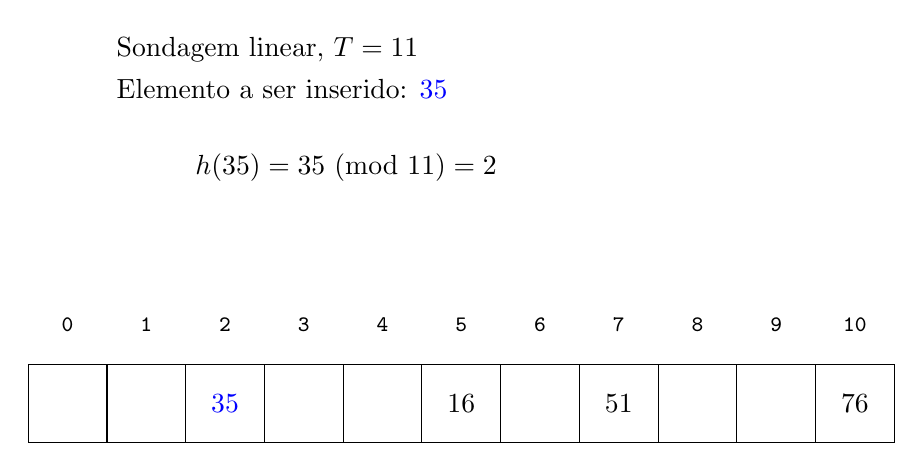
\begin{tikzpicture}
            \draw (0, 1) grid (11, 2);

            \node at (0.5, 2.5) { \tt \footnotesize 0 };
            \node at (1.5, 2.5) { \tt \footnotesize 1 };
            \node at (2.5, 2.5) { \tt \footnotesize 2 };
            \node at (3.5, 2.5) { \tt \footnotesize 3 };
            \node at (4.5, 2.5) { \tt \footnotesize 4 };
            \node at (5.5, 2.5) { \tt \footnotesize 5 };
            \node at (6.5, 2.5) { \tt \footnotesize 6 };
            \node at (7.5, 2.5) { \tt \footnotesize 7 };
            \node at (8.5, 2.5) { \tt \footnotesize 8 };
            \node at (9.5, 2.5) { \tt \footnotesize 9 };
            \node at (10.5, 2.5) { \tt \footnotesize 10 };

            \node[anchor=west] at (1, 6) { Sondagem linear, $T = 11$ };
            \node[anchor=west] at (1, 5.5) { Elemento a ser inserido: \textcolor{blue}{$35$} };

            \node[anchor=west] at (2, 4.5) { $h(35) = 35\ (\mbox{mod}\ 11) = 2$ };

            \node at (2.5, 1.5) { \textcolor{blue}{$35$} };
            \node at (5.5, 1.5) { \textcolor{black}{$16$} };
            \node at (7.5, 1.5) { \textcolor{black}{$51$} };
            \node at (10.5, 1.5) { \textcolor{black}{$76$} };
        \end{tikzpicture}
    \end{figure}

\end{frame}

\begin{frame}{Exemplo de inserção utilizando sondagem linear} 

    \begin{figure}
        \begin{tikzpicture}
            \draw (0, 1) grid (11, 2);

            \node at (0.5, 2.5) { \tt \footnotesize 0 };
            \node at (1.5, 2.5) { \tt \footnotesize 1 };
            \node at (2.5, 2.5) { \tt \footnotesize 2 };
            \node at (3.5, 2.5) { \tt \footnotesize 3 };
            \node at (4.5, 2.5) { \tt \footnotesize 4 };
            \node at (5.5, 2.5) { \tt \footnotesize 5 };
            \node at (6.5, 2.5) { \tt \footnotesize 6 };
            \node at (7.5, 2.5) { \tt \footnotesize 7 };
            \node at (8.5, 2.5) { \tt \footnotesize 8 };
            \node at (9.5, 2.5) { \tt \footnotesize 9 };
            \node at (10.5, 2.5) { \tt \footnotesize 10 };

            \node[anchor=west] at (1, 6) { Sondagem linear, $T = 11$ };
            \node[anchor=west] at (1, 5.5) { Elemento a ser inserido: \textcolor{blue}{$-6$} };

%            \node[anchor=west] at (2, 4.5) { $h(35) = 35\ (\mbox{mod}\ 11) = 2$ };

            \node at (2.5, 1.5) { \textcolor{black}{$35$} };
            \node at (5.5, 1.5) { \textcolor{black}{$16$} };
            \node at (7.5, 1.5) { \textcolor{black}{$51$} };
            \node at (10.5, 1.5) { \textcolor{black}{$76$} };
        \end{tikzpicture}
    \end{figure}

\end{frame}

\begin{frame}{Exemplo de inserção utilizando sondagem linear} 

    \begin{figure}
        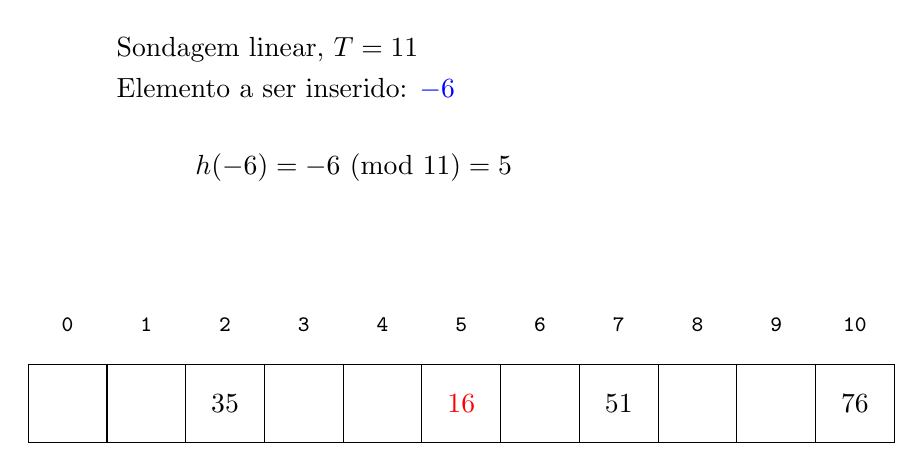
\begin{tikzpicture}
            \draw (0, 1) grid (11, 2);

            \node at (0.5, 2.5) { \tt \footnotesize 0 };
            \node at (1.5, 2.5) { \tt \footnotesize 1 };
            \node at (2.5, 2.5) { \tt \footnotesize 2 };
            \node at (3.5, 2.5) { \tt \footnotesize 3 };
            \node at (4.5, 2.5) { \tt \footnotesize 4 };
            \node at (5.5, 2.5) { \tt \footnotesize 5 };
            \node at (6.5, 2.5) { \tt \footnotesize 6 };
            \node at (7.5, 2.5) { \tt \footnotesize 7 };
            \node at (8.5, 2.5) { \tt \footnotesize 8 };
            \node at (9.5, 2.5) { \tt \footnotesize 9 };
            \node at (10.5, 2.5) { \tt \footnotesize 10 };

            \node[anchor=west] at (1, 6) { Sondagem linear, $T = 11$ };
            \node[anchor=west] at (1, 5.5) { Elemento a ser inserido: \textcolor{blue}{$-6$} };

            \node[anchor=west] at (2, 4.5) { $h(-6) = -6\ (\mbox{mod}\ 11) = 5$ };

            \node at (2.5, 1.5) { \textcolor{black}{$35$} };
            \node at (5.5, 1.5) { \textcolor{red}{$16$} };
            \node at (7.5, 1.5) { \textcolor{black}{$51$} };
            \node at (10.5, 1.5) { \textcolor{black}{$76$} };
        \end{tikzpicture}
    \end{figure}

\end{frame}

\begin{frame}{Exemplo de inserção utilizando sondagem linear} 

    \begin{figure}
        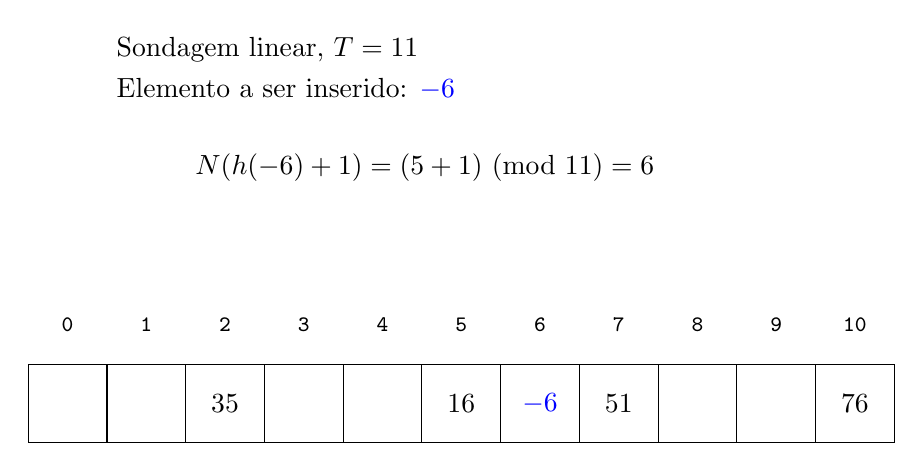
\begin{tikzpicture}
            \draw (0, 1) grid (11, 2);

            \node at (0.5, 2.5) { \tt \footnotesize 0 };
            \node at (1.5, 2.5) { \tt \footnotesize 1 };
            \node at (2.5, 2.5) { \tt \footnotesize 2 };
            \node at (3.5, 2.5) { \tt \footnotesize 3 };
            \node at (4.5, 2.5) { \tt \footnotesize 4 };
            \node at (5.5, 2.5) { \tt \footnotesize 5 };
            \node at (6.5, 2.5) { \tt \footnotesize 6 };
            \node at (7.5, 2.5) { \tt \footnotesize 7 };
            \node at (8.5, 2.5) { \tt \footnotesize 8 };
            \node at (9.5, 2.5) { \tt \footnotesize 9 };
            \node at (10.5, 2.5) { \tt \footnotesize 10 };

            \node[anchor=west] at (1, 6) { Sondagem linear, $T = 11$ };
            \node[anchor=west] at (1, 5.5) { Elemento a ser inserido: \textcolor{blue}{$-6$} };

            %\node[anchor=west] at (2, 4.5) { $h(-6) = -6\ (\mbox{mod}\ 11) = 5$ };
            \node[anchor=west] at (2, 4.5) { $N(h(-6) + 1) = (5 + 1)\ (\mbox{mod}\ 11) = 6$ };

            \node at (2.5, 1.5) { \textcolor{black}{$35$} };
            \node at (5.5, 1.5) { \textcolor{black}{$16$} };
            \node at (6.5, 1.5) { \textcolor{blue}{$-6$} };
            \node at (7.5, 1.5) { \textcolor{black}{$51$} };
            \node at (10.5, 1.5) { \textcolor{black}{$76$} };
        \end{tikzpicture}
    \end{figure}

\end{frame}

\begin{frame}{Exemplo de inserção utilizando sondagem linear} 

    \begin{figure}
        \begin{tikzpicture}
            \draw (0, 1) grid (11, 2);

            \node at (0.5, 2.5) { \tt \footnotesize 0 };
            \node at (1.5, 2.5) { \tt \footnotesize 1 };
            \node at (2.5, 2.5) { \tt \footnotesize 2 };
            \node at (3.5, 2.5) { \tt \footnotesize 3 };
            \node at (4.5, 2.5) { \tt \footnotesize 4 };
            \node at (5.5, 2.5) { \tt \footnotesize 5 };
            \node at (6.5, 2.5) { \tt \footnotesize 6 };
            \node at (7.5, 2.5) { \tt \footnotesize 7 };
            \node at (8.5, 2.5) { \tt \footnotesize 8 };
            \node at (9.5, 2.5) { \tt \footnotesize 9 };
            \node at (10.5, 2.5) { \tt \footnotesize 10 };

            \node[anchor=west] at (1, 6) { Sondagem linear, $T = 11$ };
            \node[anchor=west] at (1, 5.5) { Elemento a ser inserido: \textcolor{blue}{$49$} };

            %\node[anchor=west] at (2, 4.5) { $h(-6) = -6\ (\mbox{mod}\ 11) = 5$ };
            %\node[anchor=west] at (2, 4.5) { $N(h(-6) + 1) = (5 + 1)\ (\mbox{mod}\ 11) = 6$ };

            \node at (2.5, 1.5) { \textcolor{black}{$35$} };
            \node at (5.5, 1.5) { \textcolor{black}{$16$} };
            \node at (6.5, 1.5) { \textcolor{black}{$-6$} };
            \node at (7.5, 1.5) { \textcolor{black}{$51$} };
            \node at (10.5, 1.5) { \textcolor{black}{$76$} };
        \end{tikzpicture}
    \end{figure}

\end{frame}

\begin{frame}{Exemplo de inserção utilizando sondagem linear} 

    \begin{figure}
        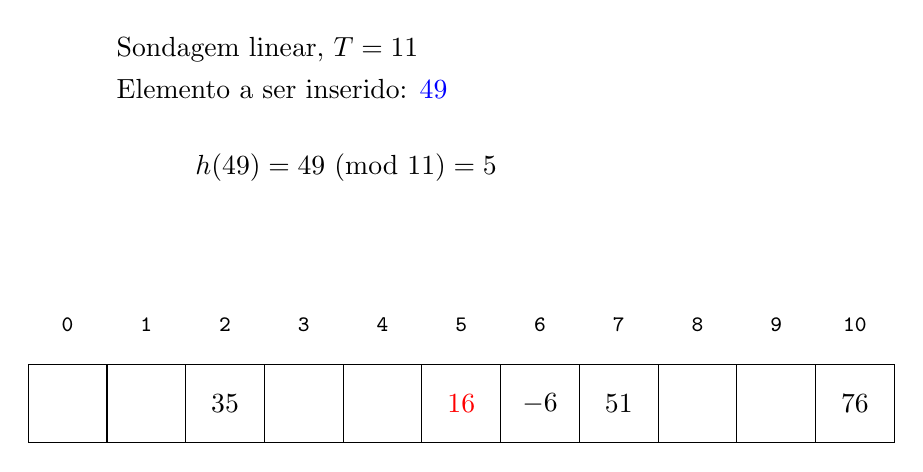
\begin{tikzpicture}
            \draw (0, 1) grid (11, 2);

            \node at (0.5, 2.5) { \tt \footnotesize 0 };
            \node at (1.5, 2.5) { \tt \footnotesize 1 };
            \node at (2.5, 2.5) { \tt \footnotesize 2 };
            \node at (3.5, 2.5) { \tt \footnotesize 3 };
            \node at (4.5, 2.5) { \tt \footnotesize 4 };
            \node at (5.5, 2.5) { \tt \footnotesize 5 };
            \node at (6.5, 2.5) { \tt \footnotesize 6 };
            \node at (7.5, 2.5) { \tt \footnotesize 7 };
            \node at (8.5, 2.5) { \tt \footnotesize 8 };
            \node at (9.5, 2.5) { \tt \footnotesize 9 };
            \node at (10.5, 2.5) { \tt \footnotesize 10 };

            \node[anchor=west] at (1, 6) { Sondagem linear, $T = 11$ };
            \node[anchor=west] at (1, 5.5) { Elemento a ser inserido: \textcolor{blue}{$49$} };

            \node[anchor=west] at (2, 4.5) { $h(49) = 49\ (\mbox{mod}\ 11) = 5$ };
            %\node[anchor=west] at (2, 4.5) { $N(h(-6) + 1) = (5 + 1)\ (\mbox{mod}\ 11) = 6$ };

            \node at (2.5, 1.5) { \textcolor{black}{$35$} };
            \node at (5.5, 1.5) { \textcolor{red}{$16$} };
            \node at (6.5, 1.5) { \textcolor{black}{$-6$} };
            \node at (7.5, 1.5) { \textcolor{black}{$51$} };
            \node at (10.5, 1.5) { \textcolor{black}{$76$} };
        \end{tikzpicture}
    \end{figure}

\end{frame}

\begin{frame}{Exemplo de inserção utilizando sondagem linear} 

    \begin{figure}
        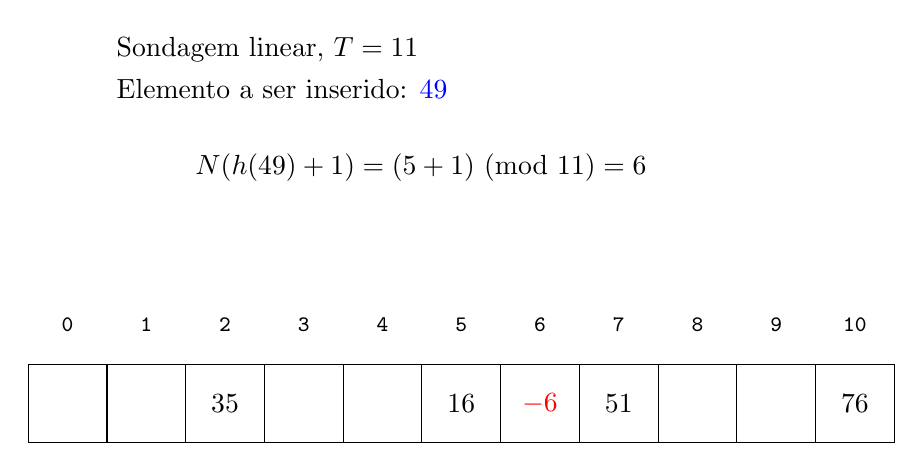
\begin{tikzpicture}
            \draw (0, 1) grid (11, 2);

            \node at (0.5, 2.5) { \tt \footnotesize 0 };
            \node at (1.5, 2.5) { \tt \footnotesize 1 };
            \node at (2.5, 2.5) { \tt \footnotesize 2 };
            \node at (3.5, 2.5) { \tt \footnotesize 3 };
            \node at (4.5, 2.5) { \tt \footnotesize 4 };
            \node at (5.5, 2.5) { \tt \footnotesize 5 };
            \node at (6.5, 2.5) { \tt \footnotesize 6 };
            \node at (7.5, 2.5) { \tt \footnotesize 7 };
            \node at (8.5, 2.5) { \tt \footnotesize 8 };
            \node at (9.5, 2.5) { \tt \footnotesize 9 };
            \node at (10.5, 2.5) { \tt \footnotesize 10 };

            \node[anchor=west] at (1, 6) { Sondagem linear, $T = 11$ };
            \node[anchor=west] at (1, 5.5) { Elemento a ser inserido: \textcolor{blue}{$49$} };

            \node[anchor=west] at (2, 4.5) { $N(h(49) + 1) = (5 + 1)\ (\mbox{mod}\ 11) = 6$ };

            \node at (2.5, 1.5) { \textcolor{black}{$35$} };
            \node at (5.5, 1.5) { \textcolor{black}{$16$} };
            \node at (6.5, 1.5) { \textcolor{red}{$-6$} };
            \node at (7.5, 1.5) { \textcolor{black}{$51$} };
            \node at (10.5, 1.5) { \textcolor{black}{$76$} };
        \end{tikzpicture}
    \end{figure}

\end{frame}

\begin{frame}{Exemplo de inserção utilizando sondagem linear} 

    \begin{figure}
        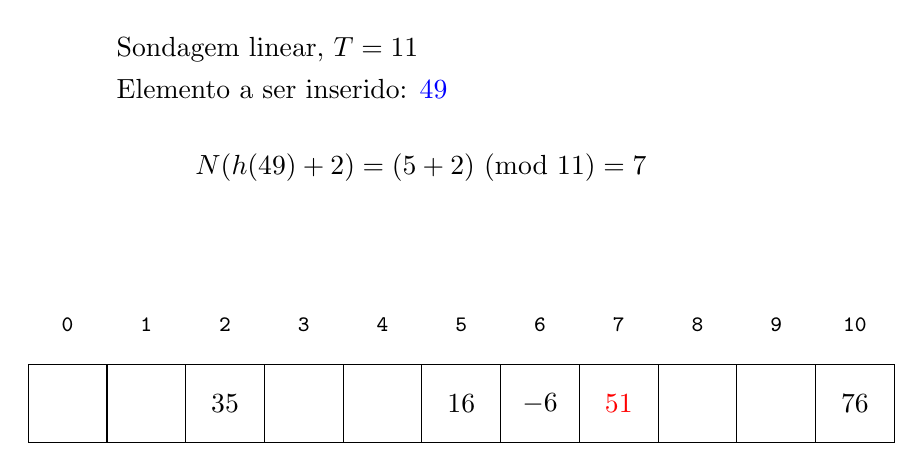
\begin{tikzpicture}
            \draw (0, 1) grid (11, 2);

            \node at (0.5, 2.5) { \tt \footnotesize 0 };
            \node at (1.5, 2.5) { \tt \footnotesize 1 };
            \node at (2.5, 2.5) { \tt \footnotesize 2 };
            \node at (3.5, 2.5) { \tt \footnotesize 3 };
            \node at (4.5, 2.5) { \tt \footnotesize 4 };
            \node at (5.5, 2.5) { \tt \footnotesize 5 };
            \node at (6.5, 2.5) { \tt \footnotesize 6 };
            \node at (7.5, 2.5) { \tt \footnotesize 7 };
            \node at (8.5, 2.5) { \tt \footnotesize 8 };
            \node at (9.5, 2.5) { \tt \footnotesize 9 };
            \node at (10.5, 2.5) { \tt \footnotesize 10 };

            \node[anchor=west] at (1, 6) { Sondagem linear, $T = 11$ };
            \node[anchor=west] at (1, 5.5) { Elemento a ser inserido: \textcolor{blue}{$49$} };

            \node[anchor=west] at (2, 4.5) { $N(h(49) + 2) = (5 + 2)\ (\mbox{mod}\ 11) = 7$ };

            \node at (2.5, 1.5) { \textcolor{black}{$35$} };
            \node at (5.5, 1.5) { \textcolor{black}{$16$} };
            \node at (6.5, 1.5) { \textcolor{black}{$-6$} };
            \node at (7.5, 1.5) { \textcolor{red}{$51$} };
            \node at (10.5, 1.5) { \textcolor{black}{$76$} };
        \end{tikzpicture}
    \end{figure}

\end{frame}

\begin{frame}{Exemplo de inserção utilizando sondagem linear} 

    \begin{figure}
        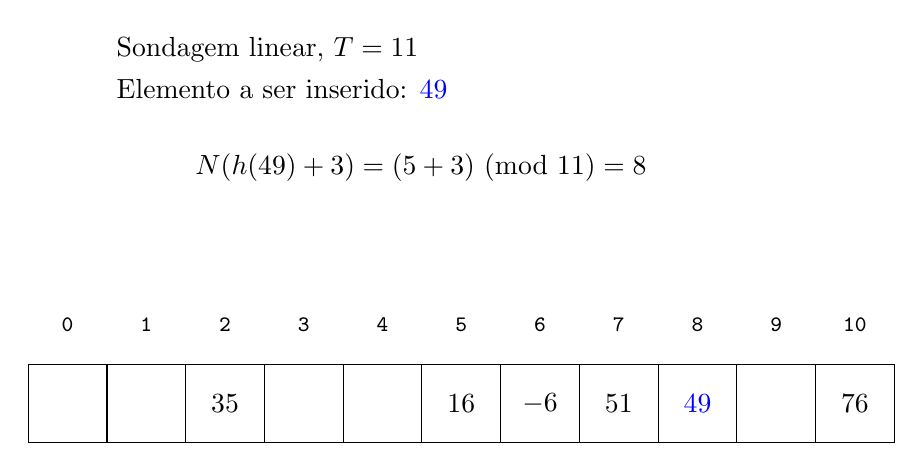
\begin{tikzpicture}
            \draw (0, 1) grid (11, 2);

            \node at (0.5, 2.5) { \tt \footnotesize 0 };
            \node at (1.5, 2.5) { \tt \footnotesize 1 };
            \node at (2.5, 2.5) { \tt \footnotesize 2 };
            \node at (3.5, 2.5) { \tt \footnotesize 3 };
            \node at (4.5, 2.5) { \tt \footnotesize 4 };
            \node at (5.5, 2.5) { \tt \footnotesize 5 };
            \node at (6.5, 2.5) { \tt \footnotesize 6 };
            \node at (7.5, 2.5) { \tt \footnotesize 7 };
            \node at (8.5, 2.5) { \tt \footnotesize 8 };
            \node at (9.5, 2.5) { \tt \footnotesize 9 };
            \node at (10.5, 2.5) { \tt \footnotesize 10 };

            \node[anchor=west] at (1, 6) { Sondagem linear, $T = 11$ };
            \node[anchor=west] at (1, 5.5) { Elemento a ser inserido: \textcolor{blue}{$49$} };

            \node[anchor=west] at (2, 4.5) { $N(h(49) + 3) = (5 + 3)\ (\mbox{mod}\ 11) = 8$ };

            \node at (2.5, 1.5) { \textcolor{black}{$35$} };
            \node at (5.5, 1.5) { \textcolor{black}{$16$} };
            \node at (6.5, 1.5) { \textcolor{black}{$-6$} };
            \node at (7.5, 1.5) { \textcolor{black}{$51$} };
            \node at (8.5, 1.5) { \textcolor{blue}{$49$} };
            \node at (10.5, 1.5) { \textcolor{black}{$76$} };
        \end{tikzpicture}
    \end{figure}

\end{frame}


\begin{frame}[fragile]{Implementação da sondagem linear}
    \inputsnippet{cpp}{1}{21}{linear.cpp}
\end{frame}

\begin{frame}[fragile]{Implementação da sondagem linear}
    \inputsnippet{cpp}{22}{41}{linear.cpp}
\end{frame}

\begin{frame}{Sondagem quadrática} 

	\begin{itemize}
		\item Na sondagem quadrática, a função de sondagem é dada por
		\[
            p(i) = (-1)^{i-1}\left\lfloor\frac{i+1}{2}\right\rfloor^2,
        \]
		para $i = 1, 2, \ldots, T - 1$

        \item A função de normalização é dada por $N(K) = K\ (\mbox{mod}\ T)$, onde $T$ é o 
            tamanho da tabela

		\item A sondagem quadrática pode ser interpretada como a sequência 
        \[
            h(K) + i^2, h(K) - i^2, h(K) + (i + 1)^2, h(K) - (i + 1)^2, \ldots
        \]
        para $i = 1, 2, \ldots, (T - 1)/2$ 

		\item Se $T$ for um número primo da forma $4k+3$, a sequência acima passa por todas 
            as posições da tabela (Radke, 1970)
	\end{itemize}

\end{frame}

\input{quadratic}

\begin{frame}[fragile]{Implementação da sondagem quadrática}
    \inputsnippet{cpp}{1}{21}{quadratic.cpp}
\end{frame}

\begin{frame}[fragile]{Implementação da sondagem quadrática}
    \inputsnippet{cpp}{23}{43}{quadratic.cpp}
\end{frame}

\begin{frame}[fragile]{\textit{hash} duplo}

    \begin{itemize}
        \item O \textit{hash} duplo é uma das melhores estratégias de endereçamento aberto

        \item Isto porque a sequência de sondagem gerada tem muitas das características das
            sequências aleatórias

        \item No \textit{hash} duplo a sequência de sondagem tem a forma
        \[
            h(K) = \Mod{(h_1(K) + ih_2(K))}{T},\ \ \ \ i=0,1,2,\ldots, T - 1
        \]
        onde $h_1(K), h_2(K)$ são duas funções de \textit{hash} auxiliares, $i$ é o índice de
        sondagem e $T$ é o tamanho da tabela

        \item Diferentemente das sondagens lineares e quadráticas, a função $h_2(K)$ depende do
            valor do chave $K$

        \item Deste modo, as sequências de sondagem para chaves $K_1\neq K_2$,
            com $h_1(K_1) = h_1(K_2)$, tendem a serem diferentes
    \end{itemize}

\end{frame}

\begin{frame}[fragile]{\textit{hash} duplo}

    \begin{itemize}
        \item A função $h_2(K)$ deve gerar valores co-primos com o tamanho $T$ da tabela

        \item Se $T$ é uma potência de dois (isto é, $T = 2^k$ para algum $k$ positivo), a
            função $h_2(K)$ deve gerar apenas números ímpares

        \item Se $T$ é um número primo, $h_2(K)$ tem que gerar números positivos menores do que
            $T$

        \item Uma maneira de se obter isso é fazer $h_1(K) = \Mod{K}{T}$ e $h_2(K) = 1 + (\Mod{K}{T - 1})$

        \item O \textit{hash} duplo tem melhor desempenho do que a sondagem linear e a sondagem
            quadrática, pois gera um número $O(T^2)$ de sondagens possíveis, enquanto que
            as outras duas geram $O(T)$ sequências de sondagem
        
    \end{itemize}

\end{frame}

\begin{frame}{Exemplo de inserção utilizando \textit{hash} duplo}

    \begin{figure}
        \begin{tikzpicture}
            \draw (0, 1) grid (11, 2);

            \node at (0.5, 2.5) { \tt \footnotesize 0 };
            \node at (1.5, 2.5) { \tt \footnotesize 1 };
            \node at (2.5, 2.5) { \tt \footnotesize 2 };
            \node at (3.5, 2.5) { \tt \footnotesize 3 };
            \node at (4.5, 2.5) { \tt \footnotesize 4 };
            \node at (5.5, 2.5) { \tt \footnotesize 5 };
            \node at (6.5, 2.5) { \tt \footnotesize 6 };
            \node at (7.5, 2.5) { \tt \footnotesize 7 };
            \node at (8.5, 2.5) { \tt \footnotesize 8 };
            \node at (9.5, 2.5) { \tt \footnotesize 9 };
            \node at (10.5, 2.5) { \tt \footnotesize 10 };

            \node[anchor=west] at (1, 6) { \textit{Hash} duplo, $T = 11$ };
            \node[anchor=west] at (1, 5.5) { Elemento a ser inserido: \textcolor{blue}{$51$} };

        \end{tikzpicture}
    \end{figure}

\end{frame}

\begin{frame}{Exemplo de inserção utilizando \textit{hash} duplo} 

    \begin{figure}
        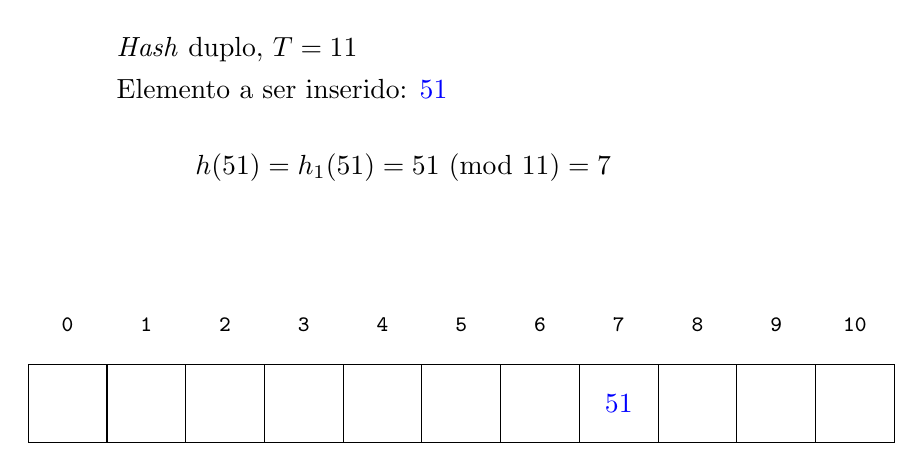
\begin{tikzpicture}
            \draw (0, 1) grid (11, 2);

            \node at (0.5, 2.5) { \tt \footnotesize 0 };
            \node at (1.5, 2.5) { \tt \footnotesize 1 };
            \node at (2.5, 2.5) { \tt \footnotesize 2 };
            \node at (3.5, 2.5) { \tt \footnotesize 3 };
            \node at (4.5, 2.5) { \tt \footnotesize 4 };
            \node at (5.5, 2.5) { \tt \footnotesize 5 };
            \node at (6.5, 2.5) { \tt \footnotesize 6 };
            \node at (7.5, 2.5) { \tt \footnotesize 7 };
            \node at (8.5, 2.5) { \tt \footnotesize 8 };
            \node at (9.5, 2.5) { \tt \footnotesize 9 };
            \node at (10.5, 2.5) { \tt \footnotesize 10 };

            \node[anchor=west] at (1, 6) { \textit{Hash} duplo, $T = 11$ };
            \node[anchor=west] at (1, 5.5) { Elemento a ser inserido: \textcolor{blue}{$51$} };

            \node[anchor=west] at (2, 4.5) { $h(51) = h_1(51) = 51\ (\mbox{mod}\ 11) = 7$ };

            \node at (7.5, 1.5) { \textcolor{blue}{$51$} };
        \end{tikzpicture}
    \end{figure}

\end{frame}

\begin{frame}{Exemplo de inserção utilizando \textit{hash} duplo} 

    \begin{figure}
        \begin{tikzpicture}
            \draw (0, 1) grid (11, 2);

            \node at (0.5, 2.5) { \tt \footnotesize 0 };
            \node at (1.5, 2.5) { \tt \footnotesize 1 };
            \node at (2.5, 2.5) { \tt \footnotesize 2 };
            \node at (3.5, 2.5) { \tt \footnotesize 3 };
            \node at (4.5, 2.5) { \tt \footnotesize 4 };
            \node at (5.5, 2.5) { \tt \footnotesize 5 };
            \node at (6.5, 2.5) { \tt \footnotesize 6 };
            \node at (7.5, 2.5) { \tt \footnotesize 7 };
            \node at (8.5, 2.5) { \tt \footnotesize 8 };
            \node at (9.5, 2.5) { \tt \footnotesize 9 };
            \node at (10.5, 2.5) { \tt \footnotesize 10 };

            \node[anchor=west] at (1, 6) { \textit{Hash} duplo, $T = 11$ };
            \node[anchor=west] at (1, 5.5) { Elemento a ser inserido: \textcolor{blue}{$16$} };

%            \node[anchor=west] at (2, 4.5) { $h(51) = 51\ (\mbox{mod}\ 11) = 7$ };

            \node at (7.5, 1.5) { \textcolor{black}{$51$} };
        \end{tikzpicture}
    \end{figure}

\end{frame}

\begin{frame}{Exemplo de inserção utilizando \textit{hash} duplo} 

    \begin{figure}
        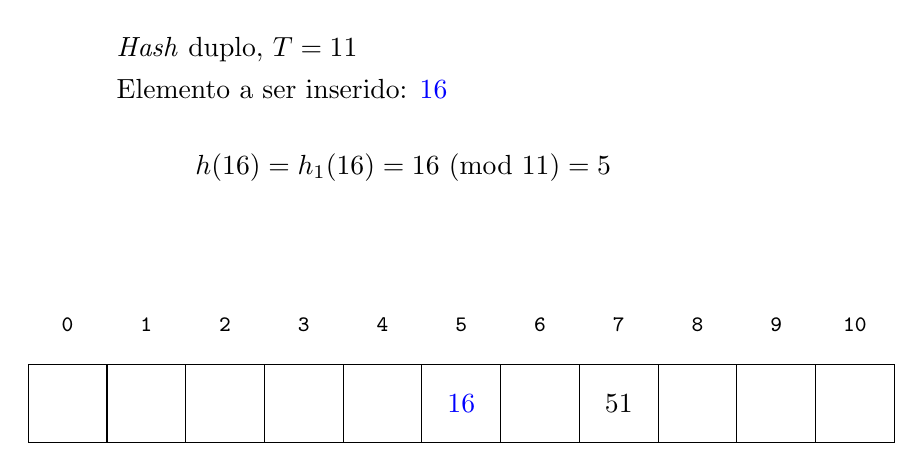
\begin{tikzpicture}
            \draw (0, 1) grid (11, 2);

            \node at (0.5, 2.5) { \tt \footnotesize 0 };
            \node at (1.5, 2.5) { \tt \footnotesize 1 };
            \node at (2.5, 2.5) { \tt \footnotesize 2 };
            \node at (3.5, 2.5) { \tt \footnotesize 3 };
            \node at (4.5, 2.5) { \tt \footnotesize 4 };
            \node at (5.5, 2.5) { \tt \footnotesize 5 };
            \node at (6.5, 2.5) { \tt \footnotesize 6 };
            \node at (7.5, 2.5) { \tt \footnotesize 7 };
            \node at (8.5, 2.5) { \tt \footnotesize 8 };
            \node at (9.5, 2.5) { \tt \footnotesize 9 };
            \node at (10.5, 2.5) { \tt \footnotesize 10 };

            \node[anchor=west] at (1, 6) { \textit{Hash} duplo, $T = 11$ };
            \node[anchor=west] at (1, 5.5) { Elemento a ser inserido: \textcolor{blue}{$16$} };

            \node[anchor=west] at (2, 4.5) { $h(16) = h_1(16) = 16\ (\mbox{mod}\ 11) = 5$ };

            \node at (5.5, 1.5) { \textcolor{blue}{$16$} };
            \node at (7.5, 1.5) { \textcolor{black}{$51$} };
        \end{tikzpicture}
    \end{figure}

\end{frame}

\begin{frame}{Exemplo de inserção utilizando \textit{hash} duplo} 

    \begin{figure}
        \begin{tikzpicture}
            \draw (0, 1) grid (11, 2);

            \node at (0.5, 2.5) { \tt \footnotesize 0 };
            \node at (1.5, 2.5) { \tt \footnotesize 1 };
            \node at (2.5, 2.5) { \tt \footnotesize 2 };
            \node at (3.5, 2.5) { \tt \footnotesize 3 };
            \node at (4.5, 2.5) { \tt \footnotesize 4 };
            \node at (5.5, 2.5) { \tt \footnotesize 5 };
            \node at (6.5, 2.5) { \tt \footnotesize 6 };
            \node at (7.5, 2.5) { \tt \footnotesize 7 };
            \node at (8.5, 2.5) { \tt \footnotesize 8 };
            \node at (9.5, 2.5) { \tt \footnotesize 9 };
            \node at (10.5, 2.5) { \tt \footnotesize 10 };

            \node[anchor=west] at (1, 6) { \textit{Hash} duplo, $T = 11$ };
            \node[anchor=west] at (1, 5.5) { Elemento a ser inserido: \textcolor{blue}{$76$} };

%            \node[anchor=west] at (2, 4.5) { $h(16) = 16\ (\mbox{mod}\ 11) = 5$ };

            \node at (5.5, 1.5) { \textcolor{black}{$16$} };
            \node at (7.5, 1.5) { \textcolor{black}{$51$} };
        \end{tikzpicture}
    \end{figure}

\end{frame}

\begin{frame}{Exemplo de inserção utilizando \textit{hash} duplo} 

    \begin{figure}
        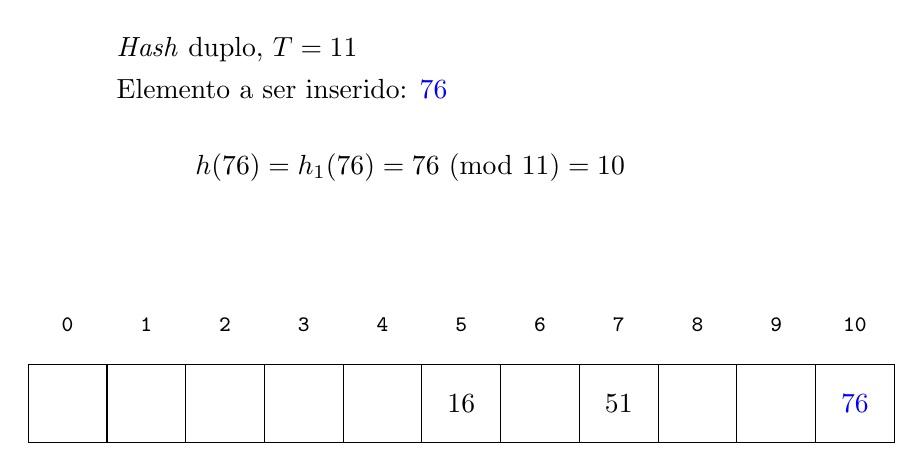
\begin{tikzpicture}
            \draw (0, 1) grid (11, 2);

            \node at (0.5, 2.5) { \tt \footnotesize 0 };
            \node at (1.5, 2.5) { \tt \footnotesize 1 };
            \node at (2.5, 2.5) { \tt \footnotesize 2 };
            \node at (3.5, 2.5) { \tt \footnotesize 3 };
            \node at (4.5, 2.5) { \tt \footnotesize 4 };
            \node at (5.5, 2.5) { \tt \footnotesize 5 };
            \node at (6.5, 2.5) { \tt \footnotesize 6 };
            \node at (7.5, 2.5) { \tt \footnotesize 7 };
            \node at (8.5, 2.5) { \tt \footnotesize 8 };
            \node at (9.5, 2.5) { \tt \footnotesize 9 };
            \node at (10.5, 2.5) { \tt \footnotesize 10 };

            \node[anchor=west] at (1, 6) { \textit{Hash} duplo, $T = 11$ };
            \node[anchor=west] at (1, 5.5) { Elemento a ser inserido: \textcolor{blue}{$76$} };

            \node[anchor=west] at (2, 4.5) { $h(76) = h_1(76) = 76\ (\mbox{mod}\ 11) = 10$ };

            \node at (5.5, 1.5) { \textcolor{black}{$16$} };
            \node at (7.5, 1.5) { \textcolor{black}{$51$} };
            \node at (10.5, 1.5) { \textcolor{blue}{$76$} };
        \end{tikzpicture}
    \end{figure}

\end{frame}

\begin{frame}{Exemplo de inserção utilizando \textit{hash} duplo} 

    \begin{figure}
        \begin{tikzpicture}
            \draw (0, 1) grid (11, 2);

            \node at (0.5, 2.5) { \tt \footnotesize 0 };
            \node at (1.5, 2.5) { \tt \footnotesize 1 };
            \node at (2.5, 2.5) { \tt \footnotesize 2 };
            \node at (3.5, 2.5) { \tt \footnotesize 3 };
            \node at (4.5, 2.5) { \tt \footnotesize 4 };
            \node at (5.5, 2.5) { \tt \footnotesize 5 };
            \node at (6.5, 2.5) { \tt \footnotesize 6 };
            \node at (7.5, 2.5) { \tt \footnotesize 7 };
            \node at (8.5, 2.5) { \tt \footnotesize 8 };
            \node at (9.5, 2.5) { \tt \footnotesize 9 };
            \node at (10.5, 2.5) { \tt \footnotesize 10 };

            \node[anchor=west] at (1, 6) { \textit{Hash} duplo, $T = 11$ };
            \node[anchor=west] at (1, 5.5) { Elemento a ser inserido: \textcolor{blue}{$35$} };

%            \node[anchor=west] at (2, 4.5) { $h(76) = 76\ (\mbox{mod}\ 11) = 10$ };

            \node at (5.5, 1.5) { \textcolor{black}{$16$} };
            \node at (7.5, 1.5) { \textcolor{black}{$51$} };
            \node at (10.5, 1.5) { \textcolor{black}{$76$} };
        \end{tikzpicture}
    \end{figure}

\end{frame}

\begin{frame}{Exemplo de inserção utilizando \textit{hash} duplo} 

    \begin{figure}
        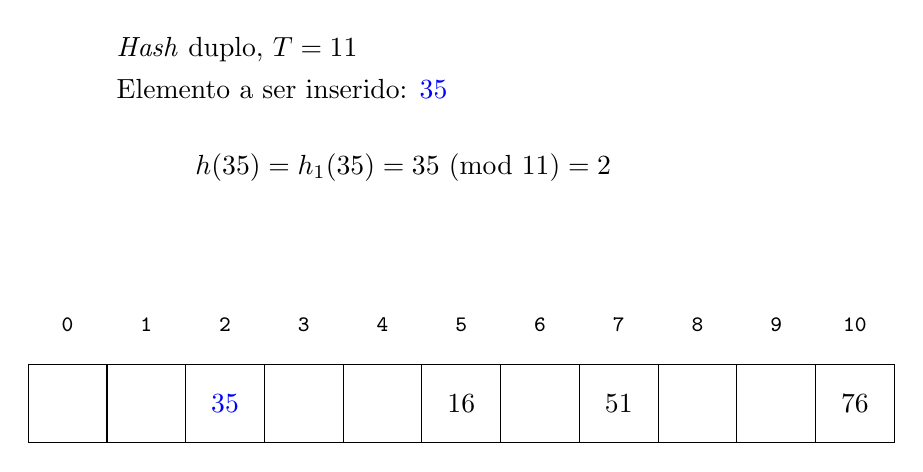
\begin{tikzpicture}
            \draw (0, 1) grid (11, 2);

            \node at (0.5, 2.5) { \tt \footnotesize 0 };
            \node at (1.5, 2.5) { \tt \footnotesize 1 };
            \node at (2.5, 2.5) { \tt \footnotesize 2 };
            \node at (3.5, 2.5) { \tt \footnotesize 3 };
            \node at (4.5, 2.5) { \tt \footnotesize 4 };
            \node at (5.5, 2.5) { \tt \footnotesize 5 };
            \node at (6.5, 2.5) { \tt \footnotesize 6 };
            \node at (7.5, 2.5) { \tt \footnotesize 7 };
            \node at (8.5, 2.5) { \tt \footnotesize 8 };
            \node at (9.5, 2.5) { \tt \footnotesize 9 };
            \node at (10.5, 2.5) { \tt \footnotesize 10 };

            \node[anchor=west] at (1, 6) { \textit{Hash} duplo, $T = 11$ };
            \node[anchor=west] at (1, 5.5) { Elemento a ser inserido: \textcolor{blue}{$35$} };

            \node[anchor=west] at (2, 4.5) { $h(35) = h_1(35) = 35\ (\mbox{mod}\ 11) = 2$ };

            \node at (2.5, 1.5) { \textcolor{blue}{$35$} };
            \node at (5.5, 1.5) { \textcolor{black}{$16$} };
            \node at (7.5, 1.5) { \textcolor{black}{$51$} };
            \node at (10.5, 1.5) { \textcolor{black}{$76$} };
        \end{tikzpicture}
    \end{figure}

\end{frame}

\begin{frame}{Exemplo de inserção utilizando \textit{hash} duplo} 

    \begin{figure}
        \begin{tikzpicture}
            \draw (0, 1) grid (11, 2);

            \node at (0.5, 2.5) { \tt \footnotesize 0 };
            \node at (1.5, 2.5) { \tt \footnotesize 1 };
            \node at (2.5, 2.5) { \tt \footnotesize 2 };
            \node at (3.5, 2.5) { \tt \footnotesize 3 };
            \node at (4.5, 2.5) { \tt \footnotesize 4 };
            \node at (5.5, 2.5) { \tt \footnotesize 5 };
            \node at (6.5, 2.5) { \tt \footnotesize 6 };
            \node at (7.5, 2.5) { \tt \footnotesize 7 };
            \node at (8.5, 2.5) { \tt \footnotesize 8 };
            \node at (9.5, 2.5) { \tt \footnotesize 9 };
            \node at (10.5, 2.5) { \tt \footnotesize 10 };

            \node[anchor=west] at (1, 6) { \textit{Hash} duplo, $T = 11$ };
            \node[anchor=west] at (1, 5.5) { Elemento a ser inserido: \textcolor{blue}{$-6$} };

%            \node[anchor=west] at (2, 4.5) { $h(35) = 35\ (\mbox{mod}\ 11) = 2$ };

            \node at (2.5, 1.5) { \textcolor{black}{$35$} };
            \node at (5.5, 1.5) { \textcolor{black}{$16$} };
            \node at (7.5, 1.5) { \textcolor{black}{$51$} };
            \node at (10.5, 1.5) { \textcolor{black}{$76$} };
        \end{tikzpicture}
    \end{figure}

\end{frame}

\begin{frame}{Exemplo de inserção utilizando \textit{hash} duplo} 

    \begin{figure}
        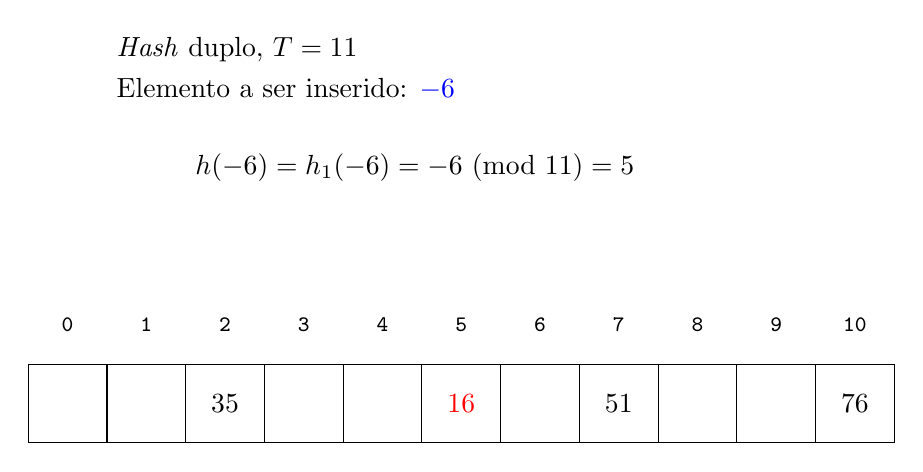
\begin{tikzpicture}
            \draw (0, 1) grid (11, 2);

            \node at (0.5, 2.5) { \tt \footnotesize 0 };
            \node at (1.5, 2.5) { \tt \footnotesize 1 };
            \node at (2.5, 2.5) { \tt \footnotesize 2 };
            \node at (3.5, 2.5) { \tt \footnotesize 3 };
            \node at (4.5, 2.5) { \tt \footnotesize 4 };
            \node at (5.5, 2.5) { \tt \footnotesize 5 };
            \node at (6.5, 2.5) { \tt \footnotesize 6 };
            \node at (7.5, 2.5) { \tt \footnotesize 7 };
            \node at (8.5, 2.5) { \tt \footnotesize 8 };
            \node at (9.5, 2.5) { \tt \footnotesize 9 };
            \node at (10.5, 2.5) { \tt \footnotesize 10 };

            \node[anchor=west] at (1, 6) { \textit{Hash} duplo, $T = 11$ };
            \node[anchor=west] at (1, 5.5) { Elemento a ser inserido: \textcolor{blue}{$-6$} };

            \node[anchor=west] at (2, 4.5) { $h(-6) = h_1(-6) = -6\ (\mbox{mod}\ 11) = 5$ };

            \node at (2.5, 1.5) { \textcolor{black}{$35$} };
            \node at (5.5, 1.5) { \textcolor{red}{$16$} };
            \node at (7.5, 1.5) { \textcolor{black}{$51$} };
            \node at (10.5, 1.5) { \textcolor{black}{$76$} };
        \end{tikzpicture}
    \end{figure}

\end{frame}

\begin{frame}{Exemplo de inserção utilizando \textit{hash} duplo} 

    \begin{figure}
        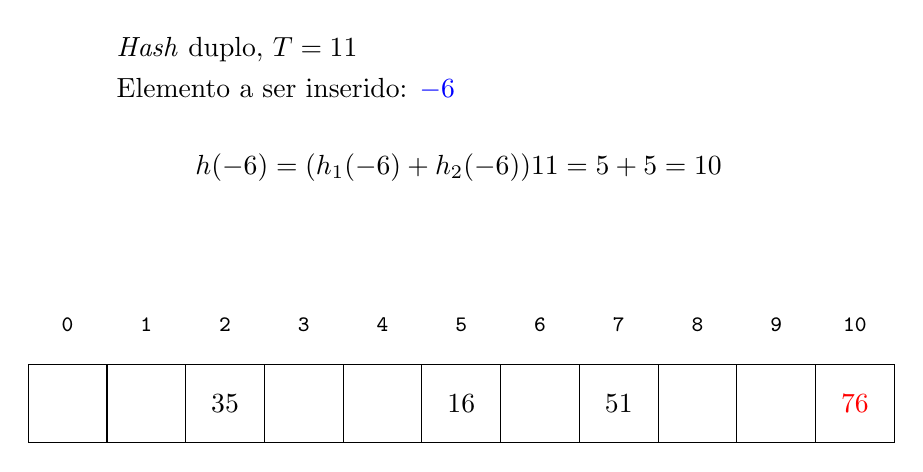
\begin{tikzpicture}
            \draw (0, 1) grid (11, 2);

            \node at (0.5, 2.5) { \tt \footnotesize 0 };
            \node at (1.5, 2.5) { \tt \footnotesize 1 };
            \node at (2.5, 2.5) { \tt \footnotesize 2 };
            \node at (3.5, 2.5) { \tt \footnotesize 3 };
            \node at (4.5, 2.5) { \tt \footnotesize 4 };
            \node at (5.5, 2.5) { \tt \footnotesize 5 };
            \node at (6.5, 2.5) { \tt \footnotesize 6 };
            \node at (7.5, 2.5) { \tt \footnotesize 7 };
            \node at (8.5, 2.5) { \tt \footnotesize 8 };
            \node at (9.5, 2.5) { \tt \footnotesize 9 };
            \node at (10.5, 2.5) { \tt \footnotesize 10 };

            \node[anchor=west] at (1, 6) { \textit{Hash} duplo, $T = 11$ };
            \node[anchor=west] at (1, 5.5) { Elemento a ser inserido: \textcolor{blue}{$-6$} };

            \node[anchor=west] at (2, 4.5) { $h(-6) = \Mod{(h_1(-6) + h_2(-6))}{11} = 5 + 5 = 10$ };

            \node at (2.5, 1.5) { \textcolor{black}{$35$} };
            \node at (5.5, 1.5) { \textcolor{black}{$16$} };
            \node at (7.5, 1.5) { \textcolor{black}{$51$} };
            \node at (10.5, 1.5) { \textcolor{red}{$76$} };
        \end{tikzpicture}
    \end{figure}

\end{frame}

\begin{frame}{Exemplo de inserção utilizando \textit{hash} duplo} 

    \begin{figure}
        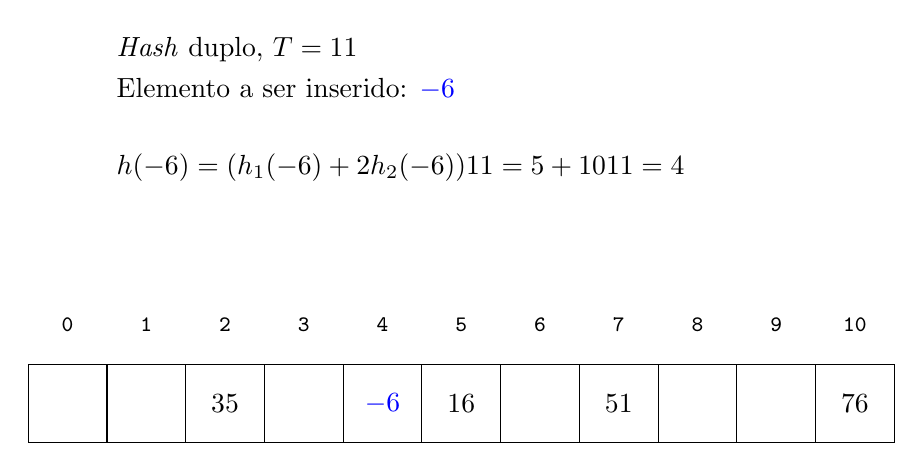
\begin{tikzpicture}
            \draw (0, 1) grid (11, 2);

            \node at (0.5, 2.5) { \tt \footnotesize 0 };
            \node at (1.5, 2.5) { \tt \footnotesize 1 };
            \node at (2.5, 2.5) { \tt \footnotesize 2 };
            \node at (3.5, 2.5) { \tt \footnotesize 3 };
            \node at (4.5, 2.5) { \tt \footnotesize 4 };
            \node at (5.5, 2.5) { \tt \footnotesize 5 };
            \node at (6.5, 2.5) { \tt \footnotesize 6 };
            \node at (7.5, 2.5) { \tt \footnotesize 7 };
            \node at (8.5, 2.5) { \tt \footnotesize 8 };
            \node at (9.5, 2.5) { \tt \footnotesize 9 };
            \node at (10.5, 2.5) { \tt \footnotesize 10 };

            \node[anchor=west] at (1, 6) { \textit{Hash} duplo, $T = 11$ };
            \node[anchor=west] at (1, 5.5) { Elemento a ser inserido: \textcolor{blue}{$-6$} };

            \node[anchor=west] at (1, 4.5) { $h(-6) = \Mod{(h_1(-6) + 2h_2(-6))}{11} = \Mod{5 + 10}{11} = 4$ };

            \node at (2.5, 1.5) { \textcolor{black}{$35$} };
            \node at (4.5, 1.5) { \textcolor{blue}{$-6$} };
            \node at (5.5, 1.5) { \textcolor{black}{$16$} };
            \node at (7.5, 1.5) { \textcolor{black}{$51$} };
            \node at (10.5, 1.5) { \textcolor{black}{$76$} };
        \end{tikzpicture}
    \end{figure}

\end{frame}


\begin{frame}{Exemplo de inserção utilizando \textit{hash} duplo} 

    \begin{figure}
        \begin{tikzpicture}
            \draw (0, 1) grid (11, 2);

            \node at (0.5, 2.5) { \tt \footnotesize 0 };
            \node at (1.5, 2.5) { \tt \footnotesize 1 };
            \node at (2.5, 2.5) { \tt \footnotesize 2 };
            \node at (3.5, 2.5) { \tt \footnotesize 3 };
            \node at (4.5, 2.5) { \tt \footnotesize 4 };
            \node at (5.5, 2.5) { \tt \footnotesize 5 };
            \node at (6.5, 2.5) { \tt \footnotesize 6 };
            \node at (7.5, 2.5) { \tt \footnotesize 7 };
            \node at (8.5, 2.5) { \tt \footnotesize 8 };
            \node at (9.5, 2.5) { \tt \footnotesize 9 };
            \node at (10.5, 2.5) { \tt \footnotesize 10 };

            \node[anchor=west] at (1, 6) { \textit{Hash} duplo, $T = 11$ };
            \node[anchor=west] at (1, 5.5) { Elemento a ser inserido: \textcolor{blue}{$49$} };

            \node at (2.5, 1.5) { \textcolor{black}{$35$} };
            \node at (4.5, 1.5) { \textcolor{black}{$-6$} };
            \node at (5.5, 1.5) { \textcolor{black}{$16$} };
            \node at (7.5, 1.5) { \textcolor{black}{$51$} };
            \node at (10.5, 1.5) { \textcolor{black}{$76$} };
        \end{tikzpicture}
    \end{figure}

\end{frame}

\begin{frame}{Exemplo de inserção utilizando \textit{hash} duplo} 

    \begin{figure}
        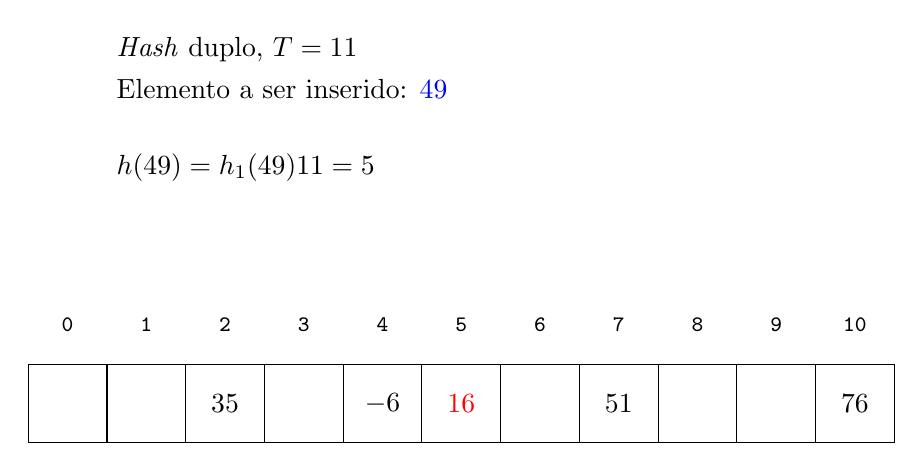
\begin{tikzpicture}
            \draw (0, 1) grid (11, 2);

            \node at (0.5, 2.5) { \tt \footnotesize 0 };
            \node at (1.5, 2.5) { \tt \footnotesize 1 };
            \node at (2.5, 2.5) { \tt \footnotesize 2 };
            \node at (3.5, 2.5) { \tt \footnotesize 3 };
            \node at (4.5, 2.5) { \tt \footnotesize 4 };
            \node at (5.5, 2.5) { \tt \footnotesize 5 };
            \node at (6.5, 2.5) { \tt \footnotesize 6 };
            \node at (7.5, 2.5) { \tt \footnotesize 7 };
            \node at (8.5, 2.5) { \tt \footnotesize 8 };
            \node at (9.5, 2.5) { \tt \footnotesize 9 };
            \node at (10.5, 2.5) { \tt \footnotesize 10 };

            \node[anchor=west] at (1, 6) { \textit{Hash} duplo, $T = 11$ };
            \node[anchor=west] at (1, 5.5) { Elemento a ser inserido: \textcolor{blue}{$49$} };

            \node[anchor=west] at (1, 4.5) { $h(49) = \Mod{h_1(49)}{11} = 5$ };

            \node at (2.5, 1.5) { \textcolor{black}{$35$} };
            \node at (4.5, 1.5) { \textcolor{black}{$-6$} };
            \node at (5.5, 1.5) { \textcolor{red}{$16$} };
            \node at (7.5, 1.5) { \textcolor{black}{$51$} };
            \node at (10.5, 1.5) { \textcolor{black}{$76$} };
        \end{tikzpicture}
    \end{figure}

\end{frame}



\begin{frame}{Exemplo de inserção utilizando \textit{hash} duplo} 

    \begin{figure}
        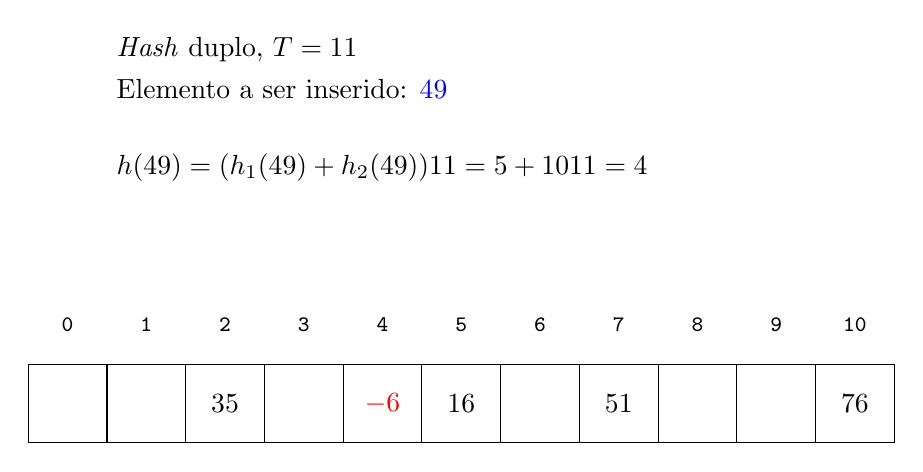
\begin{tikzpicture}
            \draw (0, 1) grid (11, 2);

            \node at (0.5, 2.5) { \tt \footnotesize 0 };
            \node at (1.5, 2.5) { \tt \footnotesize 1 };
            \node at (2.5, 2.5) { \tt \footnotesize 2 };
            \node at (3.5, 2.5) { \tt \footnotesize 3 };
            \node at (4.5, 2.5) { \tt \footnotesize 4 };
            \node at (5.5, 2.5) { \tt \footnotesize 5 };
            \node at (6.5, 2.5) { \tt \footnotesize 6 };
            \node at (7.5, 2.5) { \tt \footnotesize 7 };
            \node at (8.5, 2.5) { \tt \footnotesize 8 };
            \node at (9.5, 2.5) { \tt \footnotesize 9 };
            \node at (10.5, 2.5) { \tt \footnotesize 10 };

            \node[anchor=west] at (1, 6) { \textit{Hash} duplo, $T = 11$ };
            \node[anchor=west] at (1, 5.5) { Elemento a ser inserido: \textcolor{blue}{$49$} };

            \node[anchor=west] at (1, 4.5) { $h(49) = \Mod{(h_1(49) + h_2(49))}{11} = \Mod{5 + 10}{11} = 4 $ };

            \node at (2.5, 1.5) { \textcolor{black}{$35$} };
            \node at (4.5, 1.5) { \textcolor{red}{$-6$} };
            \node at (5.5, 1.5) { \textcolor{black}{$16$} };
            \node at (7.5, 1.5) { \textcolor{black}{$51$} };
            \node at (10.5, 1.5) { \textcolor{black}{$76$} };
        \end{tikzpicture}
    \end{figure}

\end{frame}

\begin{frame}{Exemplo de inserção utilizando \textit{hash} duplo} 

    \begin{figure}
        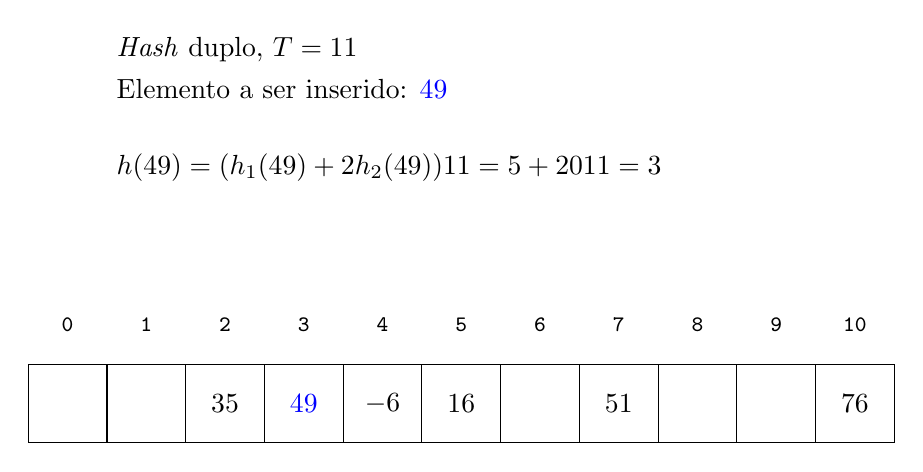
\begin{tikzpicture}
            \draw (0, 1) grid (11, 2);

            \node at (0.5, 2.5) { \tt \footnotesize 0 };
            \node at (1.5, 2.5) { \tt \footnotesize 1 };
            \node at (2.5, 2.5) { \tt \footnotesize 2 };
            \node at (3.5, 2.5) { \tt \footnotesize 3 };
            \node at (4.5, 2.5) { \tt \footnotesize 4 };
            \node at (5.5, 2.5) { \tt \footnotesize 5 };
            \node at (6.5, 2.5) { \tt \footnotesize 6 };
            \node at (7.5, 2.5) { \tt \footnotesize 7 };
            \node at (8.5, 2.5) { \tt \footnotesize 8 };
            \node at (9.5, 2.5) { \tt \footnotesize 9 };
            \node at (10.5, 2.5) { \tt \footnotesize 10 };

            \node[anchor=west] at (1, 6) { \textit{Hash} duplo, $T = 11$ };
            \node[anchor=west] at (1, 5.5) { Elemento a ser inserido: \textcolor{blue}{$49$} };

            \node[anchor=west] at (1, 4.5) { $h(49) = \Mod{(h_1(49) + 2h_2(49))}{11} = \Mod{5 + 20}{11} = 3 $ };

            \node at (2.5, 1.5) { \textcolor{black}{$35$} };
            \node at (3.5, 1.5) { \textcolor{blue}{$49$} };
            \node at (4.5, 1.5) { \textcolor{black}{$-6$} };
            \node at (5.5, 1.5) { \textcolor{black}{$16$} };
            \node at (7.5, 1.5) { \textcolor{black}{$51$} };
            \node at (10.5, 1.5) { \textcolor{black}{$76$} };
        \end{tikzpicture}
    \end{figure}

\end{frame}


\begin{frame}[fragile]{Implementação do \textit{hash} duplo}
    \inputsnippet{cpp}{1}{21}{double.cpp}
\end{frame}

\begin{frame}[fragile]{Implementação do \textit{hash} duplo}
    \inputsnippet{cpp}{23}{43}{double.cpp}
\end{frame}
